\documentclass{article}
% 11-785 Project Proposal Template
% https://www.overleaf.com/latex/templates/11-785-project-proposal-template/gvfmxtrwcttd
\usepackage{11785_project,times}
\usepackage{hyperref}
\usepackage{url}
\usepackage{graphicx}

\graphicspath{ {./img}}

\title{COMP590--171 Project Proposal: Refraction Networking}

\author{Dohhyun Kim, Harin Lim, Jesse Wei, Daniel Xie, Matseoi Zau}

\begin{document}

\maketitle

\section{Refraction networking introduction}

Refraction networking (RN) is a scheme for evading censorship technology, such as website blacklists enforced by governments, with the help of an ISP partner. Specifically, in refraction networking (also called ``decoy routing''), the user requests a blocked site, but the RN protocol actually requests a reachable site with some encrypted header information. The censoring technology accepts the legitimate request, but the ISP partner reads the header information and ``refracts'' the request to the blocked site that the user originally requested.

The specific protocol we will reimplement for our project is TapDance \cite{tapdance}.

\begin{figure}[h]
    \centering
    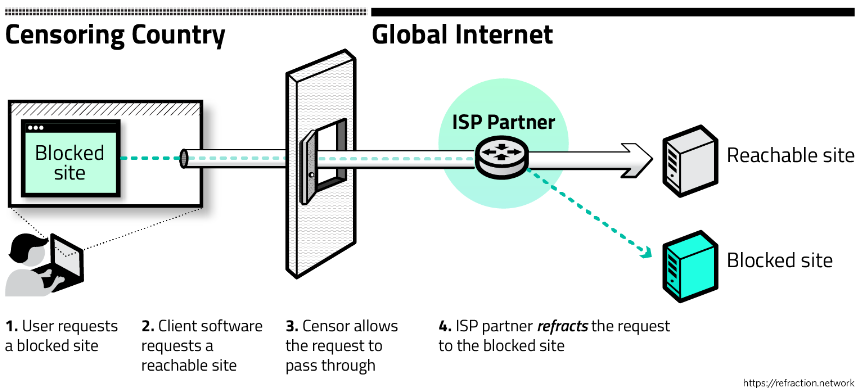
\includegraphics[width=0.8\textwidth]{refraction_networking}
    % TODO: make this not show up as [ref]
    % Note that adding author as "Refraction Network Team" makes the reference [team]
    \caption{Refraction networking \cite{refraction_network}}
\end{figure}

\section{Reimplementation of TapDance}

TODO

\section{Proof of Concept}
Now you are ready to begin the meat of your project, but you know that development will take some time. To avoid the nightmare scenario in which you spend most of your time working on an inherently flawed approach, you will need to find a toy problem or sub-problem to validate your approach(es) well before the deadline. It is also critical that the problem be simple enough such that the outcome is interpretable and the following questions (and others) can be answered:

\textit{Is it failing because of a bug in our program or because of an issue with out approach? Why isn't this strategy performing as well as we hoped? Is there a reasonable adjustment we can make to do better? Do we need to pivot?}

In this section, describe such a suitable problem and how you will evaluate the results. If applicable, list the different approaches you will be evaluating on this problem (e.g. you have two candidate algorithms for your project task).

\section{Experiments}

After you successfully evaluate your approach(es) on a smaller problem, it's now showtime. How will you move beyond this small problem and adapt your technique for the ultimate challenge? What experiments do you plan to run? This section can be less developed and speak in terms of the results of earlier experiments. You should also more thoroughly describe the setup of these final experiments and how it relates to your end goal.

\section{Member Roles}

\begin{itemize}
\item Dohhyun Kim - 
\item Harin Lim - 
\item Jesse Wei - 
\item Daniel Xie - 
\item Matseoi Zau - 
\end{itemize}


\section{Project Timeline}

\begin{itemize}
\item 2024/04/04 - Submit Proposal 
\item 2024/04/04 - Milestone 1 
\item 2024/04/04 - Milestone 2  
\item 2024/04/04 - Milestone 3  
\item 2024/05/?? - Final Presentation 
\end{itemize}
\section{Final Goals \& Evaluation}

This section should tie together the details of your experimental process and provide a metric for the successfully completed project.

\begin{itemize}
\item What do you hope to achieve by the end of the semester?
\item How will you evaluate your experiments relative to these end goals?
\item What quantitative measure are you measuring the success of your experiments by?
\item Have you decomposed your final goal into sub-goals of varying difficulty? You might say, for example, "Result \textbf{A} should be achievable based on precedent and result \textbf{B} is more ambitious. We wish to work toward \textbf{B} and report achievement on \textbf{A} first."
\end{itemize}

\section{Related Work}

Please cite blog posts, papers, projects, and other works you have consulted or plan to consult later. Please provide a sentence or two description that conveys the sources relevance to your project. You should have at least \textbf{5} sources.


\section{Data \& Technical Requirements}

Provide expected technical requirements and relevant datasets so the course staff can best support your project needs. What software libraries do you plan to use? What datasets are you using or need access to? Anything else we (the course staff) should know?

% You should cite all sources mentioned in this proposal in the file 11785_project.bib
% If you don't wish to cite some of your sources inline (e.g. in the Related Work section) using \cite{}, just you nocite to add
% them to the references section at the end of your proposal like so.
\nocite{Bengio+chapter2007}
\nocite{Hinton06}

\bibliography{refs}
\bibliographystyle{11785_project}

\end{document}
